\documentclass{article}
\usepackage{graphicx,cleveref}
\begin{document}

This report contains image differencing artefacts produced by the LSST
software stack of an older (mid Feb 2019) and of a recent  (mid May 2019)
version. 

We run \texttt{ap\_pipe.py} and \texttt{imageDifference.py} command
line tasks on the HiTS2015 dataset packaged in \texttt{ap\_verify\_hits2015}.

\section{Configuration}
There are two changes between the older and the more recent cases:
The image difference code has a bug fixed (DM-19660) which affects the
template PSF warping, thus the PSF size comparison of the images.
A new coadd template was created from the HiTS2015
dataset, which is now a direct coadd while in the older version it was
a PSF matched coadd.

Similar artefacts are produced in both the convolution and
deconvolution cases. We mainly focus on the normal convolution cases.
All configuration options were set to their software package defaults.
Gaussian base polynomial degrees are : 4,2,2. Minimum Gaussian sigma
0.7 pixel.  Fwhm scaling is enabled, sigma scaling factor (beta) is
2. For \texttt{ap\_pipe} the decorrelation afterburner was turned on
while for \texttt{imageDifference} it was not.  Unless otherwise noted
in the figure caption, pre-convolution was turned off.
%
\section{Notes}
We note the following differences between the good and bad difference
images:
\begin{itemize}
  \item The main initial observation was that fingerprint-like structures
    appear on some of the image differences. If an image is \emph{good}
    none of its sources display this characteristic pattern.
  \item In \emph{bad} difference images, most of the sources that can
    be seen on the difference image are affected. Patterns can be seen
    most conspicously in the difference sources that are bright
    sources in the original calexp.
  \item Affected sources are quite bright and may not be physical. Their
    difference flux is highly varying even in the good images.
  \item Even in a bad image, large parts of the difference image looks
    all right, most fainter sources of the calexp are properly
    subtracted.
  \item The calexps of \emph{good} difference images are taken in
    poorer conditions: have less sources and wider PSFs. The calexps
    of \emph{bad} images have more sources and sharper PSFs. Example
    PSF widths are shown in \cref{tab:psfs}.
  \item In the bad cases, higher number of sources go into the AL
    kernel solution. (About 100 in the good case vs 600 in the bad ones.) The
    circular symmetry of the pattern degrades if the number of sources
    are randomly reduced, though there remains a negative-positive
    pattern.
  \item In the bad cases, the science images are sharper, their PSF
    width is closer to the template PSF width.
  \item In the bad case, the spatial kernel solution has a highly
    oscillating profile, with positive-negative parts.
  \item Although the examples shown are all from ccd 6, it was
    verified that this was not specific to a particular ccd.
   \item The PSF resampling in DM-19660 may reduce the presence of the
     fingerprint-like pattern. Pipeline runs on larger datasets is
     part of ongoing works.  Compare \cref{fig:v410985old} and \cref{fig:v410985new}.
\end{itemize}
%
\begin{table}[h]
  \begin{center}
  \begin{tabular}{ll}
    \hline
    Visit & PSF sigma \\
    \hline
    410985 06 (sharp calexp) & 1.74 \\
    412074 06 (smoother calexp) & 2.60 \\
    411269 06 (sharp calexp) & 1.64 \\
    direct coadd template & 1.63 \\
    \hline
  \end{tabular}
  \end{center}
    \caption{\label{tab:psfs}PSF widths in the more recent dataset}
\end{table}

\begin{figure}
  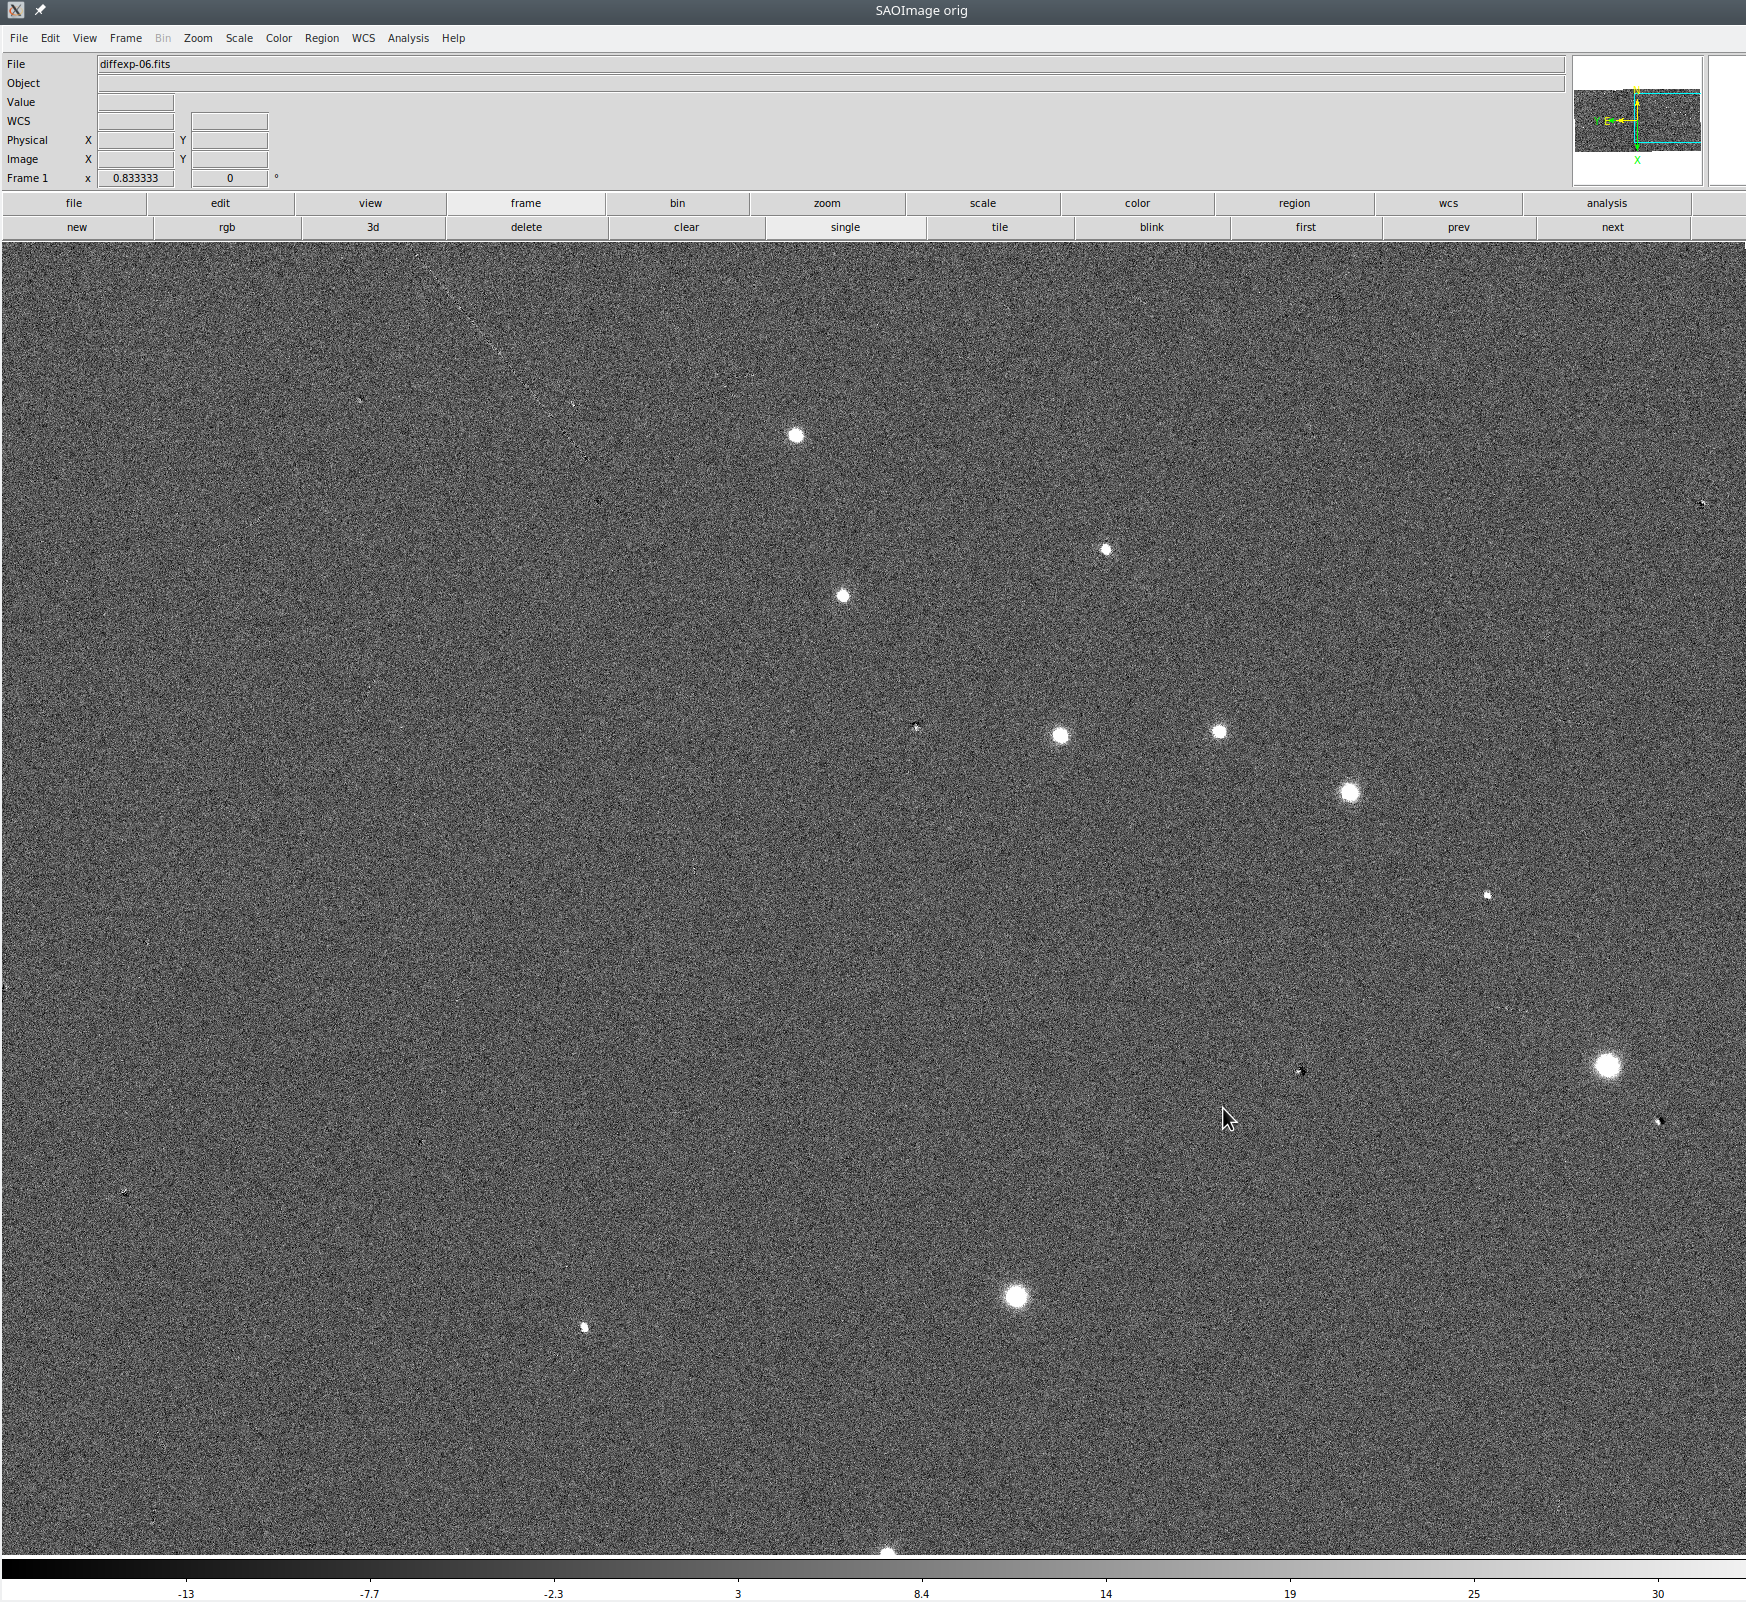
\includegraphics[width=\textwidth]{v412074_Screenshot_20190515_160748.png}
  \caption{ap\_pipe: Good subtraction case of v412074 subtracted from
    template coadd. Older case.}
\end{figure}
%
\begin{figure}
  \includegraphics[width=\textwidth]{v410985_Screenshot_20190515_154400.png}
\caption{\label{fig:v410985old}ap\_pipe: Bad subtraction case of v410985 subtracted from
  template coadd. Older case.}  
\end{figure}
%
\begin{figure}
  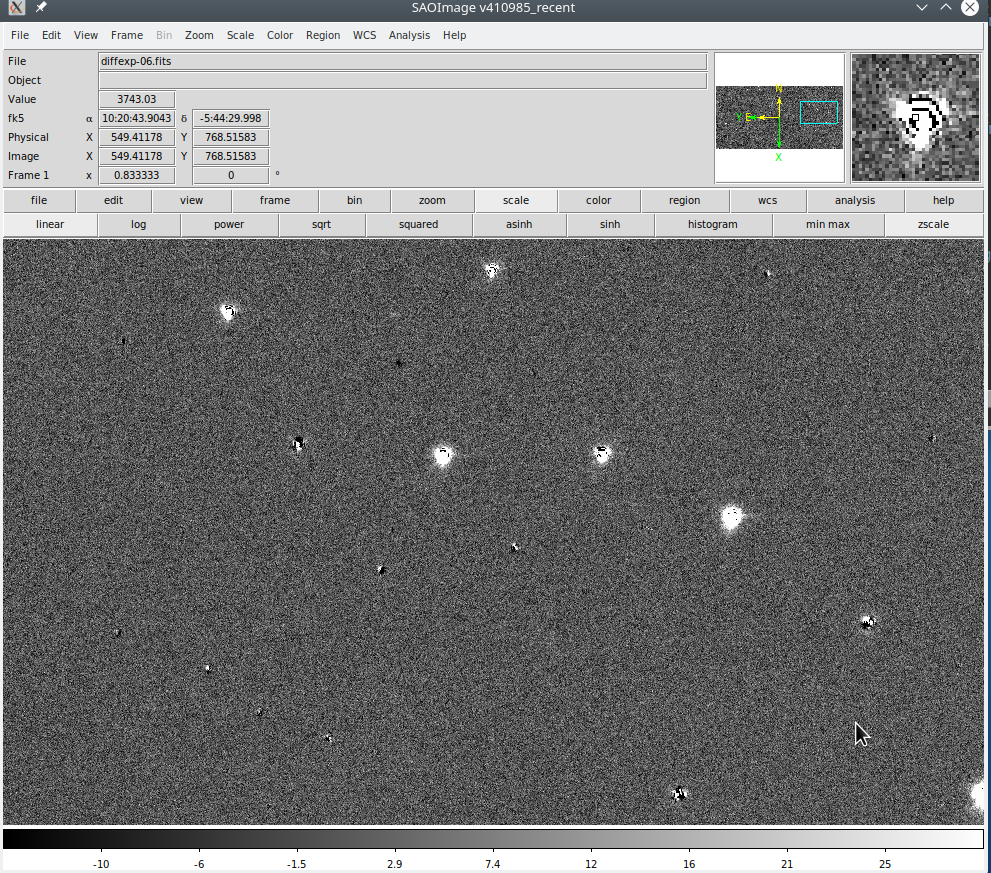
\includegraphics[width=\textwidth]{Scr_v410985_recent.png}
\caption{\label{fig:v410985new}imageDifference: Bad subtraction case of v410985 ccd 6 subtracted from
  template coadd. Recent case.}  
\end{figure}
%
\begin{figure}
  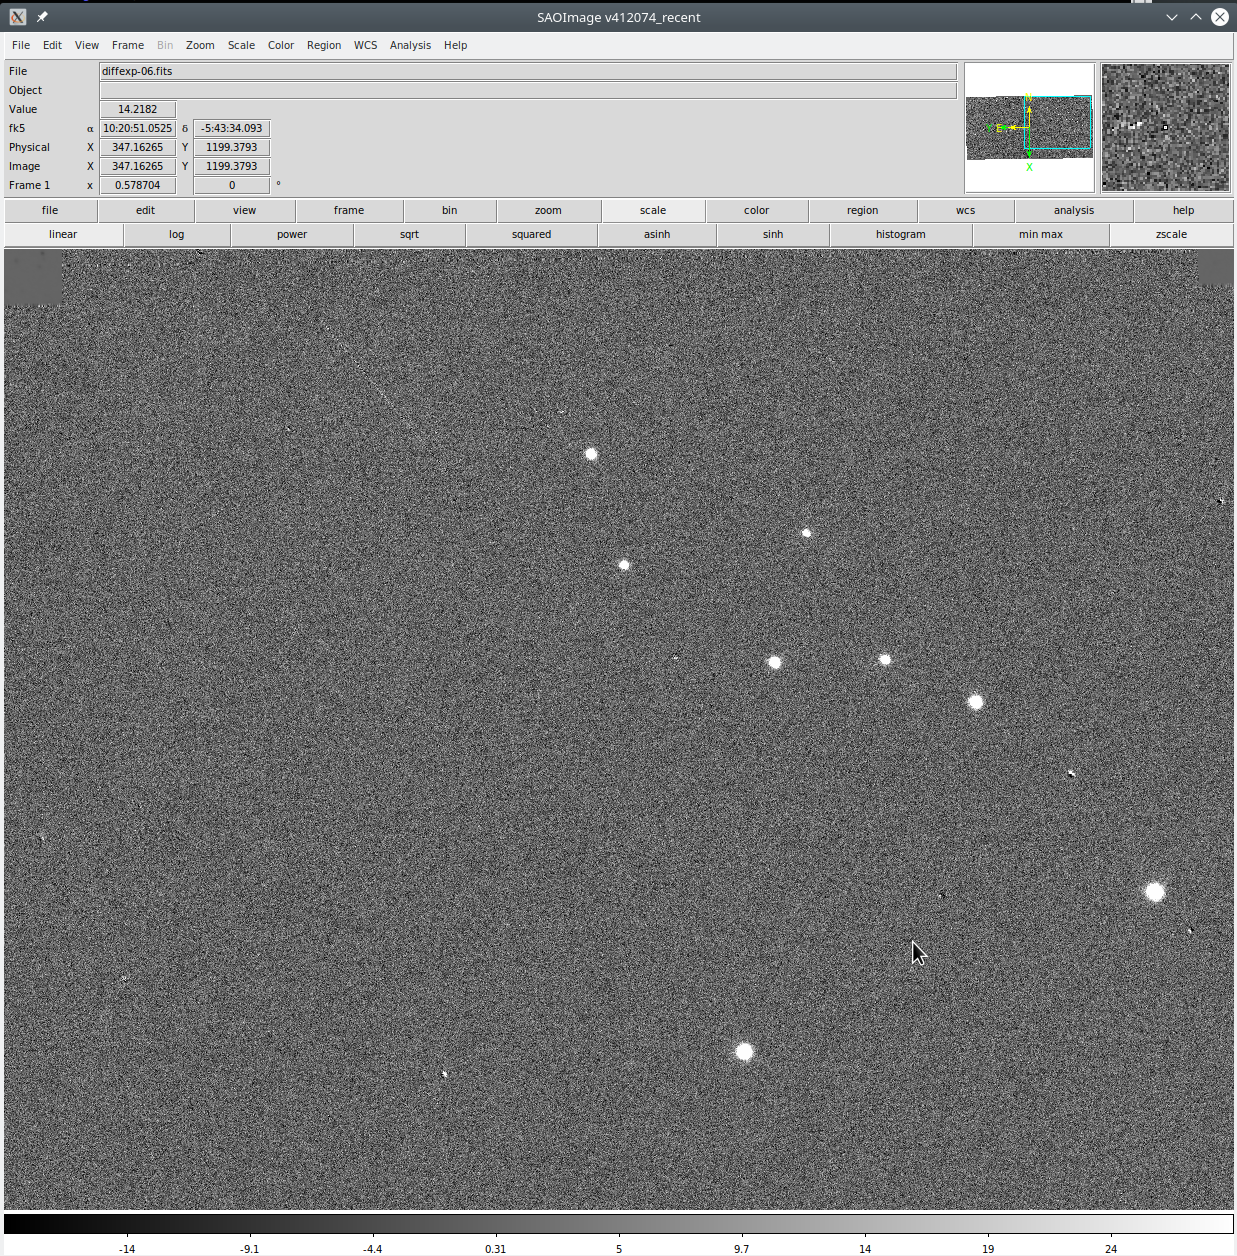
\includegraphics[width=\textwidth]{Scr_v412074_recent.png}
\caption{ImageDifference: Good subtraction case of v412074 ccd 6 subtracted from
  template coadd. Recent case.}  
\end{figure}
%
\begin{figure}
  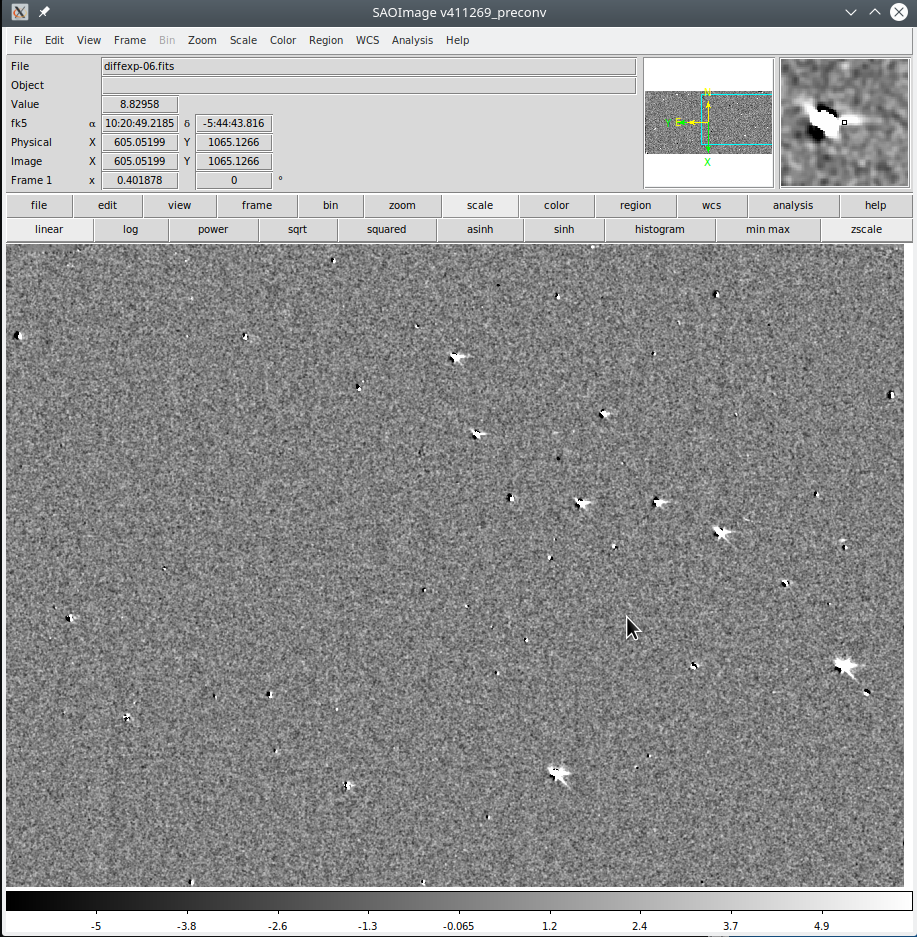
\includegraphics[width=\textwidth]{Scr_v411269_preconv.png}
\caption{imageDifference: Subtraction of sharp calexp v411269 from template with Gaussian
  preconvolution. Recent version.}
\end{figure}
%
\begin{figure}
  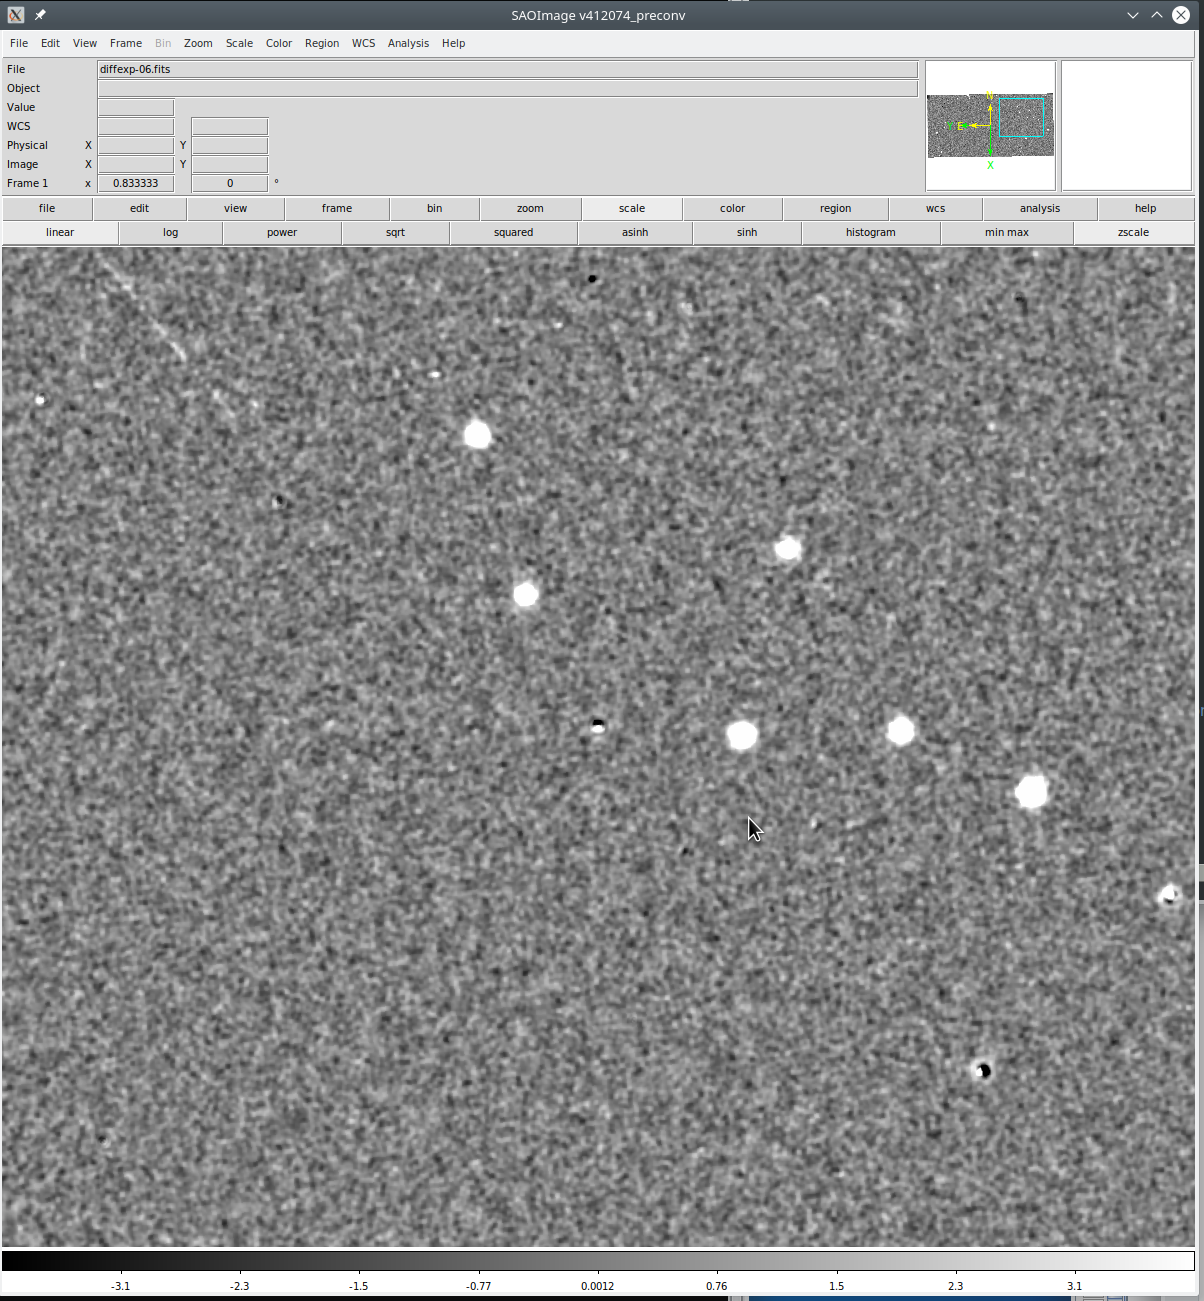
\includegraphics[width=\textwidth]{Scr_v412074_preconv.png}
\caption{imageDifference: Subtraction of a smoother calexp (v412074) from template with Gaussian
  preconvolution. Recent version.}
\end{figure}
%
In \cref{fig:calexps412074,fig:calexps410985} we show direct calexp subtractions.
\begin{figure}
  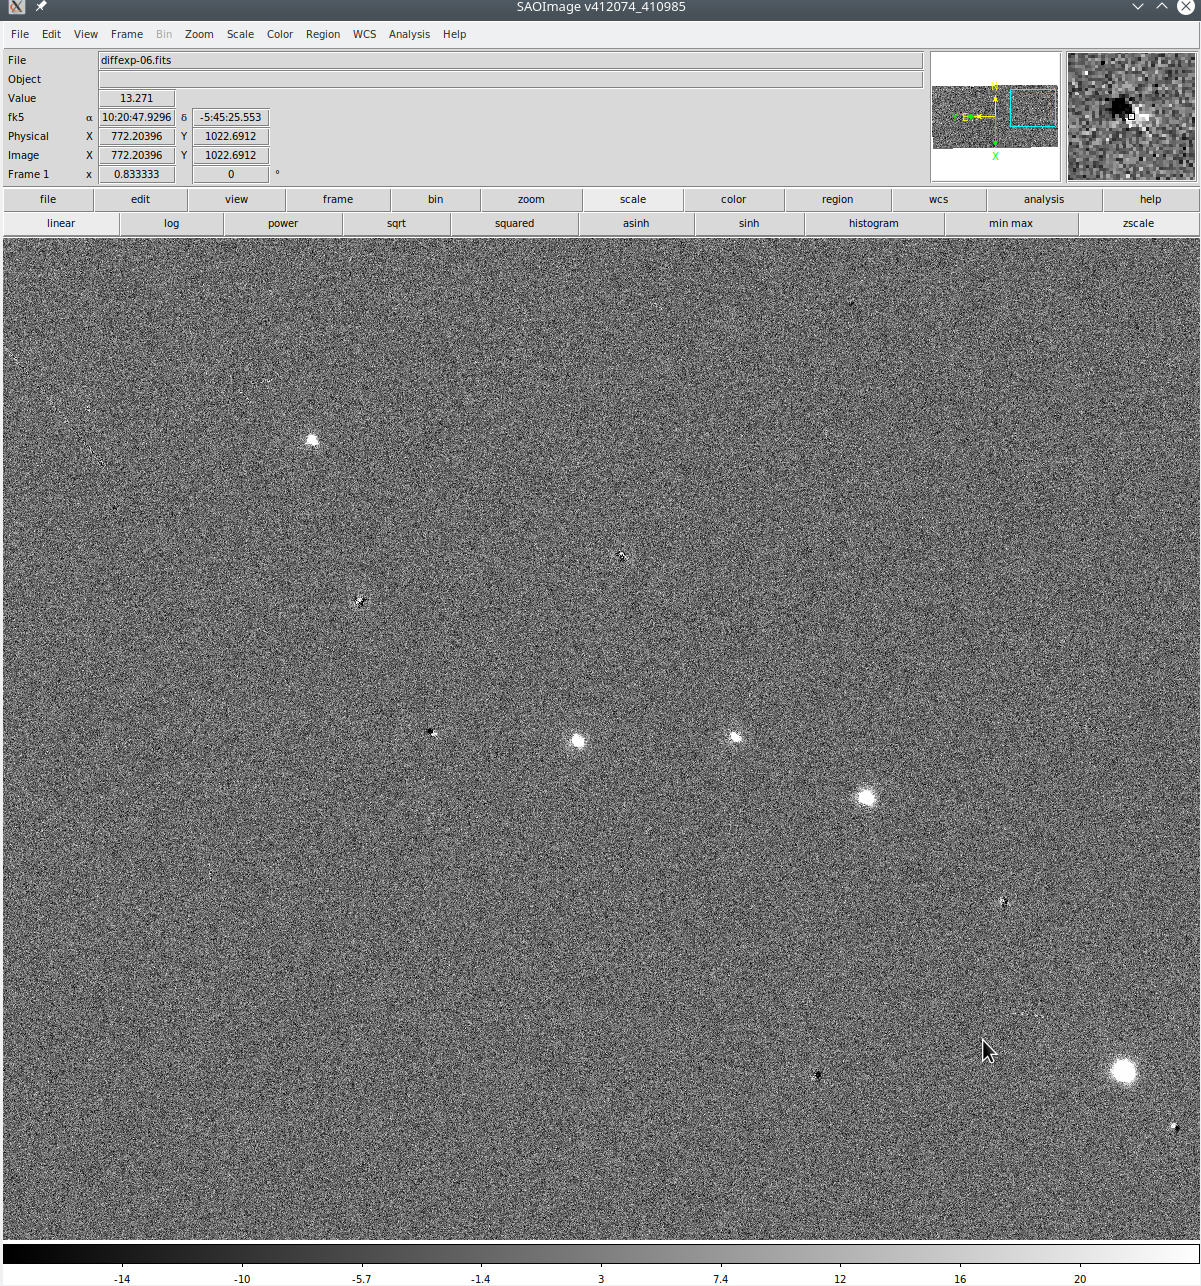
\includegraphics[width=\textwidth]{Scr_412074_410985_calexps.png}
  \caption{\label{fig:calexps412074}imageDifference: Subtracting two
    calexps: a sharper (v410985) image from a smoother (v412074) one.}
\end{figure}
%
\begin{figure}
  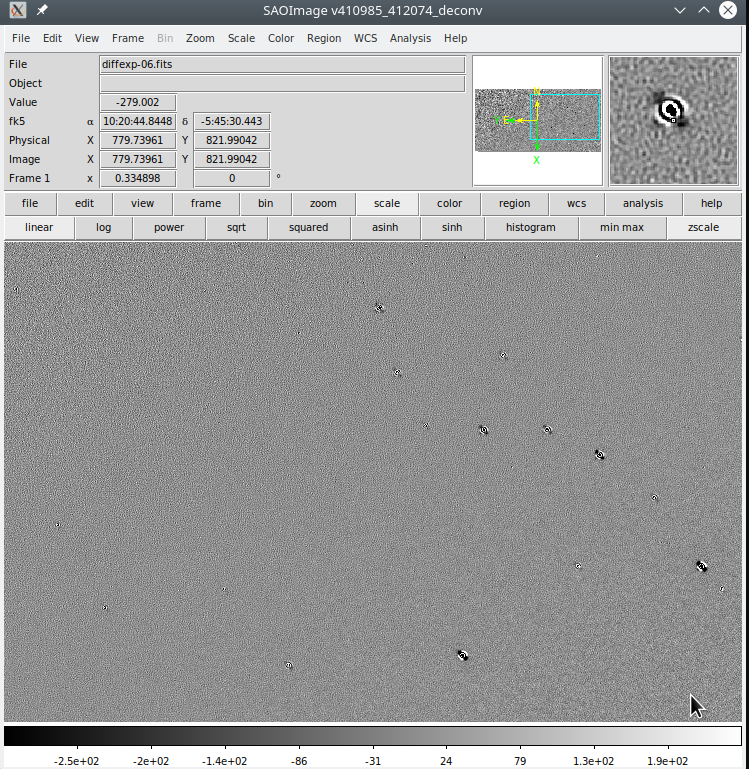
\includegraphics[width=\textwidth]{Scr_v410985_412074_deconv_calexps.png}
  \caption{\label{fig:calexps410985}imageDifference: Subtracting two calexps,
    deconvolution case: a smoother (v412074) image from a sharper
    (v410985) one.}
\end{figure}
% 
\end{document}